% !iTeXMac(input): POH.tex
\chapter{AIRPLANE HANDLING, SERVICE \& MAINTENANCE} \vspace{\minitocspacebefore} \minitoc \cleardoublepage

\section{INTRODUCTION} This is a place-holder for the Airplane Handling, Service \& Maintenance Section. The section will be completed once in-service experience has been gained.

\section{GROUND HANDLING}
Ground motion is best accomplished by pushing or pulling on the propeller as near to the
spinner as possible. The following are recommended additional pushing locations to help move the
airplane: 

\begin{itemize*}
  \item Moving forward --- front seat support (canopy open).
  \item Moving rearwards --- wing leading edges and roots of horizontal stabilizer.
  \end{itemize*}

A suitable pushbar may be fitted over the two ends of the tailwheel axle.

Take care to not use high power during run-up, as the tail will lift even if the control stick is held full aft.

Wing tie down mounting points are located centrally under each wing. Use a 3/8" dia x 16
tpi eye bolt to attach tie down rope to airplane. Secure a third line to the tail wheel spring.

\subsection{Canopy Protection and Ventilation}
If the aircraft is tied down outdoors and subject to weather elements for any length of time, then the use of an aircraft canopy cover is highly recommended. The cover will protect canopies and windows from abrasive dust, dirt, and sand kicked up by wind or prop wash. Before purchasing, verify that the canopy cover is NOT waterproof as the trapped moisture and heat from the sun can be deleterious. Acrylic subjected to this treatment over a period of time may turn slightly milky and eventually crazes.

Keep the canopy ventilated or covered when the aircraft is parked in the hot sun. Cabin temperatures can easily reach 150-200 degrees F even on a mild day. The acrylic can generally take these temperature conditions multiple times without any apparent adverse effect, but the cumulative affect that will cause shortened service life. The use of a canopy cover will significantly reduce the internal temperatures inside the aircraft to just a few degrees above outside ambient temperatures. Additionally it will also protect the avionics from heat and the upholstery/seat belt harnesses from harmful UV rays.

\section{SERVICING}
\subsection{Brakes}
The brake fluid reservoir is located on the engine side of the firewall near the upper left side.  The preferred brake fluid is MIL-PRF-83282, but MIL-H-5606 fluid can mixed if required.  Note that MIL-H-5606 has a much lower flash point, so should be avoided if possible.

The original O-rings in the brake calipers were replaced with Viton O-rings, due to the much higher acceptable temperature of Viton.

\section{CLEANING AND CARE}
\subsection{Windscreen and Canopy}
The windscreen and canopy are fabricated from polymethyl methacrylate) (PMMA), an acrylic plastic, brand name Plexiglas.

\subsubsection{Cleaning}
For general cleaning use Dawn dishwashing liquid or equivalent and water followed by a clear water rinse. To prevent water spots, blow dry with compressed air or wipe dry with soft cotton flannel. Plexus, Sprayaway \#848 Industrial Plastic Cleaner, or All Clear can also be used for day to day cleaning. Grease, oil, tape residue, etc. may best be removed with Mineral spirits, refined kerosene, white gasoline, naphtha, or isopropyl alcohol. Wash approved solvents off of canopy with Dawn dishwashing liquid and water. It is best to avoid using products that are not specifically formulated for acrylics (such as Rain-X or Lemon Pledge) on the canopy.

\begin{Note}[CAUTION]DO NOT use Loctite, aromatic solvents, acetone, benzene, ethyl acetate, carbon tetrachloride, lighter fluid, lacquer thinners, gasoline, toluene, window sprays, concentrated alcohols, keytones, scouring compounds, ammonia, or 409 cleaner on or around acrylic canopy materials.
\end{Note}

\subsubsection{Scratch Removal}
Small scratches can be buffed out with Meguiar's Mirror Glaze \#17. For deep scratch removal, use Scratch Off , Micro Mesh, or 3M Window Repair kits. Avoid removing scratches in critical areas where clear visibility is important, as the process will usually result in some degree of optical distortion.

\section{COWLING REMOVAL} 
\begin{enumerate*}
  \item Open oil filler door and remove the two pins that secure the aft edge of the top cowling to the firewall.
  \item Remove the two triangular stainless steel plates that cover the forward end of the pins that join the top and bottom cowlings at the horizont split line (Torx T15 driver needed).
  \item Use a small screwdriver or punch in the pin loops to remove the pins that secure the horizontal split line.
  \item Remove the six Phillips screws that join the top and bottom cowlings just behind the spinner.
  \item Pull the aft, lower edges of the top cowling outwards to disengage the hinge loops at the aft edge and along the aft portion of the horizontal split line.
  \item Lift the forward end of the top cowling slightly, then remove the Torx T15 screws that secure the aft edge of the upper air inlet ducts to the cooling plenum (three scews on right side and four on left side).
  \item Remove the top cowling, lifting with one hand in the oil filler door and the other hand on the front of the top cowling.
  \item Remove the two short pins that secure the aft edge of the bottom cowling to the firewall.
  \item Remove the pin that secures the aft edge of the left side of the bottom cowling to the firewall.
  \item Pull the left, aft edge of the bottom cowling outwards to disengage the hinge loops.
  \item Remove the pin that secures the aft edge of the right side of the bottom cowling to the firewall.
  \item Pull the right, aft edge of the bottom cowling outwards to disengage the hinge loops.
  \item Remove the bottom cowling.
  \end{enumerate*}


\section{INSPECTION PANELS}
In addition to the engine cowling, the aircraft has a number of inspection and access panels:
\begin{enumerate*}
  \item Oil dipstick access door on aft right side of upper cowling.
  \item Instrument panel access door on aft wall of forward baggage compartment. Four Torx T10 screws are removed, allowing the access panel to be opened.
  \item Three under-wing inspection panels on each wing provide access to fuel tank securing bolts and aileron bellcranks.
  \item Rear fuselage inspection plates on each side provide access to the elevator horns.
  \item Rear baggage compartment aft wall and hat shelf are removable, providing access to the battery and rear fuselage.
  \item Cockpit and rear baggage compartment floors are removable.
  \item Wing tips are removable, but note that they must remain close to the wing tips due to the coax connections to an internal antenna in each wing tip, and the power wires for the strobe and navigation lights in each wing tip.
  \end{enumerate*}

\begin{Note}[CAUTION]
The ADS-B must not be powered up unless an ADS-B antenna is connected to it.  If the middle right wing inspection panel is removed, and it is desired to power up the aircraft, either:
\begin{enumerate*}
	\item Remove the fuse for the ADS-B transmitter, or
	\item Uplug the wiring harness from Echo UAT ADS-B transmitter, on the bottom of the avionics shelf below the instrument panel, or
	\item Connect the ADS-B antenna to its coax.
\end{enumerate*}
\end{Note}

\needspace{10\baselineskip}
\section{INITIAL INSPECTIONS}

The following inspections are required following first flight:

\subsection{After First Flight} 
\begin{enumerate*}
	\item Complete firewall forward detailed visual inspection. 
	\item Check alternator belt tension (7 -- 9 ft-lb on pulley when belt slips). 
	\item Complete airframe visual detailed inspection. 
\end{enumerate*}

%\subsection{2 Hours} 
%\begin{enumerate*}
%	\item Lubricate propeller hub. See 100 Hour Inspection or Hartzell Propeller Owner's Manual for details of procedure. 
%\end{enumerate*}

\subsection{10 Hours} 
\begin{enumerate*}
	\item Change oil, cut open oil filter and inspect, and inspect suction screen. Look for metal particles, shavings or flakes. Info from Lycoming Service Bulletin No. 480D, July 13, 2000. 
	\item Retorque landing gear bolts.
	\item Complete items from Conditional Inspection, except for oil change, propeller lubrication, ELT. 
\end{enumerate*}

\subsection{25 Hours} 
\begin{enumerate*}
	\item Check alternator belt tension (7 -- 9 ft-lb on pulley when belt slips). 
\end{enumerate*}

\subsection{35 Hours} 
\begin{enumerate*}
	\item Change oil, cut open oil filter and inspect, and inspect suction screen. Look for metal particles, shavings or flakes. Info from Lycoming Service Bulletin No. 480D, July 13, 2000. 
	\item Complete items from Conditional Inspection, except for oil change, propeller lubrication, ELT. 
\end{enumerate*}

\section{PERIODIC MAINTENANCE} This section includes all items specified in the Lycoming Owner's Manual and MT Operation and Installation manual. It is supplemented by recommendations from Van's Aircraft, other RV owners, and engineering judgement.

\subsection{50 Hours or 4 months} The following items should be performed every 50 hours, or four months, whichever comes first:
\begin{enumerate*}
	\item Drain oil sump with oil hot. Send sample for analysis (see Lycoming Service Letter No. 171). 
	\item Replace oil filter. Cut open \& inspect. 
	\item Inspect \& clean suction oil screen. 
	\item Check \& record brake fluid level. 
	\item Check integrity of: 
	\begin{enumerate*}
		\item Fuel \& oil hoses, 
		\item Ignition system, 
		\ifthenelse{\thePMAG = 0}{\item Magneto P-lead \& mounting bolts, }{\item PMag wiring at connector \& mounting bolts}
		\item Exhaust system \& attachment hardware, 
		\item Cylinders - check for oil leak at rocker box covers, and check for signs of overheating (burned paint), 
		\item Baffling/plenum, 
		\item Firewall forward wiring, 
		\item Engine mount bolts, 
		\item Firewall seals, and 
		\item Cowling hinge eyes. 
	\end{enumerate*}
	\item Inspect \& lubricate: 
	\begin{enumerate*}
		\item Throttle, mixture \& prop linkages, 
		\item Alternate air door \& control, and 
		\item Oil cooler door \& control. 
		\item Tail wheel (disassemble, inspect locking pin for burrs, lubricate and reassemble) 
	\end{enumerate*}
	\item Check alternator belt condition \& tension. 
	\item Check tires for wear, rotate/replace as necessary. 
	\item On test flight, log engine data. 
\end{enumerate*}

\subsection{100 Hours or 12 months} The following items should be performed every 100 hours, or 12 months, whichever comes first: 
\begin{enumerate*}
	\item Complete the items from the 50 hour inspection, plus 
	\item Remove, clean, inspect and regap spark plugs.
	\item Inspect \& clean gascolator screen. 
	\item Inspect \& clean fuel filter. \textcolor{red}{Check recommended interval.} 
	\item Conduct compression check on all cylinders. 
	\item Propeller 
	\begin{enumerate*}
		\item Remove spinner 
		\item Inspect spinner and back plate. 
		\item Check propeller mounting bolts and safety wire. 
		\item Inspect prop blades for nicks and cracks. 
		\item Inspect prop hub for cracks or grease leakage. \textcolor{red}{Add any items from MT manuals}. 
		\item Check blade track. 
		\begin{enumerate*}
			\item Chock the wheels securely. 
			\item Place a fixed reference point beneath the propeller, within 0.25" below the lowest point of the propeller arc. Fasten a sheet of paper to the reference point. 
			\item Rotate the propeller by hand (opposite the direction of normal rotation) until a blade points directly at the paper. Mark the position of the blade tip on the paper. 
			\item Repeat the procedure with the second blade. 
			\item Tracking tolerance is 0.125" between the position of the two blades. 
		\end{enumerate*}
		\item Reinstall the spinner. 
	\end{enumerate*}
	\item Check alternator belt tension (7 -- 9 ft-lb on pulley when belt slips). 
\ifthenelse{\thePMAG = 1}{
	\item PMag Electronic Ignition
	\begin{enumerate*}
		\item Check E-Mag website for Service Bulletin compliance.
		\item Check PMag thermal sticker for exceedence. 
		\item Check PMag ignition lead resistance is approximately $180\Omega$ per foot.  Confirm the resistance is approximately stable while bending, twisting and tugging each end.
		\item Check PMag plug gaps.
		\item Remove PMag and check for smooth rotation and no excessive lateral or axial play in shaft. 
		\item Torque wire lead connection screws to 5 in--lb.
		\item Set PMag timing. 
	\end{enumerate*}}
{	\item Magneto
	\begin{enumerate*}
		\item Check breaker points for pitting and minimum gap, 
		\item Check for excessive oil in breaker compartment, 
		\item Lubricate breaker point felt, and 
		\item Check Magneto to Engine timing. See Lycoming Direct Drive Overhaul Manual for details of procedure.
	\end{enumerate*}}
	\item Light Speed Electronic Ignition
	  \begin{enumerate*}
	    \item Remove Hall Effect Sensor and open up to check for gear, bearing and seal wear
	    \item Set electronic ignition timing
    	\end{enumerate*} 	
	\item Check cylinders visually for cracked or broken fins, 
	\item Check engine mounting bolts and bushings, 
	\item Check fuel injector nozzles for looseness, tighten to 60 in-lb torque, 
	\item Check fuel lines for dye stains at connections, and 
	\item Re-install spark plugs with new washers. 
\end{enumerate*}

\subsection{400 Hours} The following items should be performed every 400 hours: 
\begin{enumerate*}
	\item Replace spark plugs, and 
	\item Remove rocker box covers and check for freedom of valve rockers when valves are closed. Look for evidence of abnormal wear or broken parts in the area of valve tips, valve keeper, springs and spring seats. 
\end{enumerate*}

\subsection{500 Hours} The following items should be performed every 500 hours or 36 months:
\begin{enumerate*}
\ifthenelse{\thePMAG = 0}{\item\textcolor{red}{Insert Slick's recommended items.}}{}
	\item Light Speed Electronic Ignition: 
	\begin{enumerate*}
		\item Replace high tension leads (i.e. coil to spark plug wires), and 
	\end{enumerate*}
\end{enumerate*}

\subsection{1500 Hours} The following items should be performed every 1500 hours or 10 years (from CAR 625 Appendix C --- not mandatory for amateur-built aircraft). MT's recommended overhaul interval is 1800 hrs or 72 months.
\begin{enumerate*}
	\item Overhaul propeller. 
\end{enumerate*}

\subsection{3 Months} The ELT Self Test must be performed every 3 months.  See ELT SELF-TEST later in this section.

\subsection{12 Months} The following items must be performed every 12 months (the due date is exactly 12 months following the previous inspection):
\begin{enumerate*}
	\item Conduct compass swing of any non-stabilized magnetic compass and install dated compass card (requirement from CAR 625 App. C).
	\item Inspect ELT (requirement from CAR 625 App. C).
\end{enumerate*}

\subsection{24 Months} The following items must be performed every 24 months (the due date is exactly 24 months following the previous inspection):
\begin{enumerate*}
	\item Calibrate altimeter and altitude encoder IAW AWM 571 App. B (requirement from CAR 625 App. C).
	\item Test transponder IAW AWM 571 App. F (requirement from CAR 625 App. C).
\end{enumerate*}

\section{ANNUAL INSPECTION} An annual inspection must be carried out once every 12 months (the due date is the end of the 12th month following the previous inspection). The inspection must include all items listed in CAR 625 Appendix B. The following list expands on the required items. Items marked with (*) are not required as per CAR 625 Appendix B. Completion of these items is not required as per the CARs, but is strongly recommended to improve reliability and safety.

\begin{enumerate*}
	\item{AD Review}
	\begin{enumerate*}
		\item Print list of applicable ADs from TC web site.\dotfill $\bigbox$
		\item Comply with ADs during inspection as required.\dotfill $\bigbox$
	\end{enumerate*}

  \item{Aircraft General}
  \begin{enumerate*}
    \item Remove or open all inspection panels, access doors, fairings and cowlings. \dotfill $\bigbox$
    \item Thoroughly clean the aircraft. \dotfill $\bigbox$
    \item Inspect panel, door and cowling closing and locking mechanisms for improper installation, function and condition. \dotfill $\bigbox$
		\end{enumerate*}

	\item{Engine} 
\ifthenelse{\thePMAG = 1}{\begin{Note}[WARNING] \centering Ground PMag before working on engine. \end{Note}}
{\begin{Note}[WARNING] \centering Ground mags before working on engine. \end{Note}}
	\begin{enumerate*}
		\item Remove engine cowl.\dotfill $\bigbox$
		\item Cowling --- clean it and inspect for cracks, distortion and loose or missing fasteners.\dotfill $\bigbox$
		\item Leaks --- inspect engine, oil lines and oil cooler for oil leaks.\dotfill $\bigbox$
		\item Oil 
		\begin{enumerate*}
			\item Oil temp. sender --- inspect for leaks and security. \dotfill $\bigbox$
			\item Oil lines and fittings --- inspect for leaks, chafing security, dents and cracks. \dotfill $\bigbox$
			\item Oil cooler --- clean cooling fins and inspect condition. (*)\dotfill $\bigbox$
			\item Screens and sump drain plugs --- inspect for metal particles and foreign matter. \dotfill $\bigbox$
			\item Fill engine with oil per \textcolor{red}{lubrication chart}. \dotfill $\bigbox$
		\end{enumerate*}
		\item Ignition (*)
		\begin{enumerate*}
			\item Check condition of spark plugs and adjust gap. \dotfill $\bigbox$
			\item Check ignition harness and insulators. \dotfill $\bigbox$
\ifthenelse{\thePMAG = 0}{\item Check magneto points for proper clearance maintain at \textcolor{red}{.018 $\pm $ .006}. \dotfill $\bigbox$
			\item Check magneto for oil seal leaks. \dotfill $\bigbox$
			\item Check breaker felt for proper lubrication. \dotfill $\bigbox$
			\item Check distributor block for cracks, burned areas or corrosion. \dotfill $\bigbox$
			\item Check magnetos to engine timing. See Lycoming Direct Drive Overhaul Manual for details of procedure. \dotfill $\bigbox$}
			{\item Check E-Mag website for Service Bulletin compliance. \dotfill $\bigbox$
			\item Check PMag thermal sticker for exceedence. \dotfill $\bigbox$
			\item Check PMag ignition lead resistance is approximately $180\Omega$ per foot.  Confirm the resistance is approximately stable while bending, twisting and tugging each end.  \dotfill $\bigbox$
			\item Remove PMag and check for smooth rotation and no excessive lateral or axial play in shaft. \dotfill $\bigbox$
			\item Torque PMag wire lead connection screws to 5 in--lb. \dotfill $\bigbox$
			\item Set PMag timing. \dotfill $\bigbox$}
			\item Remove Light Speed electronic ignition Hall Effect Sensor and open up to check for gear, bearing and seal wear. \dotfill $\bigbox$
			\item Set Light Speed electronic ignition timing. \dotfill $\bigbox$
		\end{enumerate*}
		\item Thoroughly clean engine and other items ahead of the firewall. \dotfill $\bigbox$
		\item Studs and nuts --- inspect for defects, evidence of improper torque and safety locking. \dotfill $\bigbox$
  	\item Cylinder compression --- conduct compression check on all cylinders. Record readings: \\* \hfill \#1:\underline{\makebox[0.5in][l]{}} \\* \hfill \#2:\underline{\makebox[0.5in][l]{}} \\* \hfill \#3:\underline{\makebox[0.5in][l]{}} \\* \hfill \#4:\underline{\makebox[0.5in][l]{}} \\* If compression test indicates problems, check internal condition and tolerances. \dotfill $\bigbox$
		\item Remove air filter and clean. \dotfill $\bigbox$
		\item Check condition of alternate air door and cable. \dotfill $\bigbox$
		\item Fuel Injection System
		\begin{enumerate*}
  		\item Inspect fuel injection servo. \dotfill $\bigbox$
  		\item Inspect condition of fuel injection lines IAW FAA AD 2011-26-04 \& Lycoming MSB 342G. \dotfill $\bigbox$
		\end{enumerate*}
		\item Clean screens in fuel pump. \dotfill $\bigbox$
		\item General condition: \dotfill $\bigbox$
		\begin{enumerate*}
		\item Check engine controls throttle, carb heat, mixture, prop and alternate air door. Check condition, proper travel and safety locking. \dotfill $\bigbox$
		\item Exhaust system --- inspect for cracks, defects and improper attachment. \dotfill $\bigbox$
		\item Inspect heater muffs, heater boxes and SCAT tubes. \dotfill $\bigbox$
		\item Check breather tube for obstructions and security. \dotfill $\bigbox$
		\item Check crankcase for cracks, leaks, security of bolts. \dotfill $\bigbox$
		\item Engine mounts --- inspect for cracks, looseness of mounting and looseness of engine to mount. \dotfill $\bigbox$
		\item Flexible vibration dampeners --- inspect for poor condition and deterioration. \dotfill $\bigbox$
		\item Check all engine baffles and plenum parts. \dotfill $\bigbox$
		\item Check firewall seals. \dotfill $\bigbox$
		\item Check condition and tension of alternator, alternator mount, drive belt and B-lead. \dotfill $\bigbox$
		\item Check condition of starter, starter mount, starter cable and solenoid. \dotfill $\bigbox$
		\item Inspect all starter power and ground connections ahead of firewall and clean as necessary. \dotfill $\bigbox$
		\item Check standby alternator. \dotfill $\bigbox$
		\item Check prop governor. \dotfill $\bigbox$
		\item Internal corrosion --- inspect engines which have not been inhibited and have been out of \\service in excess of 12 months. \dotfill $\bigbox$
	  \end{enumerate*}
		\item Check \& record brake fluid level. (*) \dotfill $\bigbox$
		\item Lubricate all controls. \dotfill $\bigbox$
		\item Reinstall engine cowl. \dotfill $\bigbox$
	\end{enumerate*}
	\item{Fuel System} 
	\begin{enumerate*}
		\item Clean and inspect fuel filter. \dotfill $\bigbox$
		\item Clean and inspect gascolator. \dotfill $\bigbox$
		\item Inspect condition of fuel lines. \dotfill $\bigbox$
		\item Check fuel system for leaks. \dotfill $\bigbox$
		\item Check pressure from electric fuel pump is 25 -- 45 psi. Record pressure: \underline{\makebox[0.5in][l]{}} \dotfill $\bigbox$
		\item Check operation of fuel selector valve. \dotfill $\bigbox$
		\item Check fuel vents. \dotfill $\bigbox$
	\end{enumerate*}

	\item{Propeller} 
	\begin{enumerate*}
	  \item Propeller hub assembly --- inspect for cracks, nicks, binding and oil leakage. \dotfill $\bigbox$
	  \item Bolts and nuts --- inspect for improper torque and safety locking. \dotfill $\bigbox$
	  \item Control mechanisms --- inspect for improper operation, insecure mounting and improper range of \\travel. \dotfill $\bigbox$
	  \item Composite blades --- inspect for:
	  \begin{enumerate*}
	    \item cracks, bruises, scars, warping, evidence of glue failure and delamination, \dotfill $\bigbox$
	    \item attachment bolt tightness, and \dotfill $\bigbox$
	    \item correct track, excessive rotational and end play. \dotfill $\bigbox$

  	  \end{enumerate*}
  	\item Spinner assembly --- inspect for cracks and wear. \dotfill $\bigbox$
  	\item Variable pitch propellers --- check correct operation during ground run. \dotfill $\bigbox$
	\end{enumerate*}


	\item{Cockpit} 
	\begin{enumerate*}
		\item Remove seats and cockpit floors. \dotfill $\bigbox$
		\item Generally --- inspect for dirt and loose equipment that might foul the controls. \dotfill $\bigbox$
		\item Inspect cockpit area, forward fuselage and underfloor area for corrosion, cracks, chafed wiring, deterioration, distortion, evidence of failure, defective or insecure attachment fittings, etc. \dotfill $\bigbox$
		\item Check for dirt and loose equipment that might foul the controls. \dotfill $\bigbox$
		\item Check all wing front spar attachment bolts. \dotfill $\bigbox$
		\item Check rear spar carry through structure. \dotfill $\bigbox$
		\item Inspect COM 1 and transponder antennae and coax. \dotfill $\bigbox$
		\item Landing gear boxes --- inspect condition of wiring, etc. Check for FOD. \dotfill $\bigbox$
		\item Landing gear attach bolts --- Check torque \dotfill $\bigbox$
		\item Controls:
  	\begin{enumerate*}
  		\item Check control columns, systems and connection. \dotfill $\bigbox$
  		\item Lubricate control column bearings as required. \dotfill $\bigbox$
  		\item Check pitch and roll trim operation from front and rear seats. \dotfill $\bigbox$
  		\item Check flap motor, wiring and pushrods. \dotfill $\bigbox$
  		\item Lubricate flap pushrod bearings as required. \dotfill $\bigbox$
  	  \end{enumerate*}
		\item Reinstall cockpit floors and front seat. \dotfill $\bigbox$
		\item Windscreen and canopy --- inspect for deterioration and breakage. \dotfill $\bigbox$
		\item Windscreen and canopy --- inspect canopy tracks, rollers and latch. \dotfill $\bigbox$
		\item Canopy Latch --- disassemble, inspect, lubricate and reassemble. \dotfill $\bigbox$
		\item Upholstery --- inspect for security and tears. (*) \dotfill $\bigbox$
		\item Seats and safety belts --- inspect for poor condition, fraying, and any other apparent defects. \dotfill $\bigbox$
		\item Rudder pedals, brake cylinders, parking brake valve and brake lines --- check condition. \dotfill $\bigbox$
		\item Gooseneck and instrument lights --- check condition and function of lamps and dimmers. \dotfill $\bigbox$
		\item Instrument Panel:
  	\begin{enumerate*}
  		\item Instruments --- inspect for poor condition, mounting, marking and, where practicable, for \\improper operation. \dotfill $\bigbox$
  		\item Placards ---- confirm all placards listed in the POH are in place and are legible. \dotfill $\bigbox$
  		\item Static System --- conduct static system leak check. (*) \dotfill $\bigbox$
      \end{enumerate*}
		\item Check condition of heater controls. \dotfill $\bigbox$
		\item Check condition of throttle, mixture and propeller speed controls. \dotfill $\bigbox$
		\item Check condition of oil cooler door and alternate air controls. \dotfill $\bigbox$
		\item Check condition and operation of air vents. \dotfill $\bigbox$
		\item Check fire extinguisher. \dotfill $\bigbox$
		\item Check wire bundles for chafing, paying particular attention to Infinity stick grip wire bundle at \\bottom of stick. \dotfill $\bigbox$
	\end{enumerate*}
	\item{Aft Fuselage} 
	\begin{enumerate*}
		\item Remove aft baggage floor and aft baggage rear bulkhead. \dotfill $\bigbox$
		\item Check under whole aft fuselage, including skins, bulkheads, longerons, stiffeners ,under baggage floor area for corrosion, cracks, chafed wiring, deterioration, distortion, evidence of failure, defective or insecure attachment fittings, etc. \dotfill $\bigbox$
		\item Battery --- inspect for improper installation and improper charge. Inspect battery hold-down and \\battery cables. Check battery voltage with no load. \dotfill $\bigbox$
		\item Strobe power supply --- Check condition and wiring. \dotfill $\bigbox$
		\item GPS antenna --- check condition of antenna and coax cable. \dotfill $\bigbox$
		\item Elevator bellcrank and elevator control tubes --- check condition. Lubricate bellcrank and \\pushrod ends as required. \dotfill $\bigbox$
		\item Reinstall aft baggage floor and aft baggage rear bulkhead. \dotfill $\bigbox$
	\end{enumerate*}
  \item{ELT} 
  \begin{enumerate*}
  	\item Inspect mounting tray and fasteners. \dotfill $\bigbox$
  	\item Inspect coax cable for abrasion. Disconnect coax connections and inspect jack and plug for corrosion. \dotfill $\bigbox$
  	\item Inspect cable to remote control for abrasion. Disconnect connections and inspect for corrosion. \dotfill $\bigbox$
  	\item Inspect GPS data cable for abrasion. Disconnect GPS data cable and inspect jack and plug for \\corrosion. \dotfill $\bigbox$
  	\item Check expiration date of ELT, aural alert and remote batteries and replace if they will expire \\within the next 12 months. \dotfill $\bigbox$
  	\item Conduct g-switch test from FAA Order 8250.3. From ACK manual, page 13. (*) \dotfill $\bigbox$
  	\begin{enumerate*}
  		\item Remove ELT from tray. \dotfill $\bigbox$
  		\item Select ELT switch to ARMED. \dotfill $\bigbox$
  		\item Monitor 121.5, with squelch turned OFF. \dotfill $\bigbox$
  		\item During first five minutes of the hour, test g-switch: 
  		\begin{enumerate*}
  		  \item hold the ELT at your waist with the arrow printed on the battery case facing away from you. \dotfill $\bigbox$
  		  \item move the ELT rapidly away from your waist. \dotfill $\bigbox$
  		  \item when the ELT reaches the full extent of your arm retract it back to your waist as fast \\as possible. \dotfill $\bigbox$
  		  \end{enumerate*} 
  		\item Verify that the ELT tone is heard. \dotfill $\bigbox$
  		\item Select ELT switch to OFF within 30 s (406 MHz emergency signal is sent 50 s after g-switch activation). \dotfill $\bigbox$
  	\end{enumerate*}
  	\item Reinstall ELT \dotfill $\bigbox$
  	\item Set ELT switch to ARMED \dotfill $\bigbox$
  	\item Replace red guard over ELT switch \dotfill $\bigbox$
  	\item Reseal DIN connector with tape \dotfill $\bigbox$
  	\item Perform ELT Self Test, due every three months \dotfill $\bigbox$
  \end{enumerate*}
	\item{Empennage} 
	\begin{enumerate*}
		\item Remove empennage fairing and elevator horn inspection covers. \dotfill $\bigbox$
		\item Check horizontal stabilizer attachment. \dotfill $\bigbox$
		\item Check vertical fin attachments. \dotfill $\bigbox$
		\item Check vertical fin and rudder surfaces. \dotfill $\bigbox$
		\item Check rudder horn and attachment. \dotfill $\bigbox$
		\item Check rudder bolts for wear. \dotfill $\bigbox$
		\item Check rudder strobe and nav light for security. \dotfill $\bigbox$
		\item Check horizontal stabilizer and elevators. \dotfill $\bigbox$
		\item Inspect horizontal stabilizer front spar IAW SB 14-01-31. \dotfill $\bigbox$
		\item Record SB 14-01-31 inspection in logbook. \dotfill $\bigbox$
		\item Check elevator trim tab and servo. \dotfill $\bigbox$
		\item Check elevator horn. \dotfill $\bigbox$
		\item Check elevator bolts for wear. \dotfill $\bigbox$
		\item Inspect elevator spar IAW SB 14-02-05. \dotfill $\bigbox$
		\item Record SB 14-02-05 inspection in logbook. \dotfill $\bigbox$
		\item Lubricate all bearings as needed. \dotfill $\bigbox$
		\item Reinstall empennage fairing and elevator horn inspection covers. \dotfill $\bigbox$
	\end{enumerate*}
	\item{Wings} 
	\begin{enumerate*}
		\item Remove wing root fairing and under-wing inspection panels. \dotfill $\bigbox$
		\item Check fuel tank to fuselage mount. \dotfill $\bigbox$
		\item Check wing rear spar attachment bolts. \dotfill $\bigbox$
		\item Check surfaces for damage and loose rivets. \dotfill $\bigbox$
		\item Check wing walk condition. \dotfill $\bigbox$
		\item Check flaps and pushrods. \dotfill $\bigbox$
		\item Check fuel tank bolts on front spar. \dotfill $\bigbox$
		\item Check aileron bellcrank and control tubes. \dotfill $\bigbox$
		\item Inspect rear wing spar for cracks IAW SB 16-03-28. \dotfill $\bigbox$
		\item Record SB 16-03-28 inspection in logbook. \dotfill $\bigbox$
		\item Lubricate aileron bellcrank and pushrods as required. \dotfill $\bigbox$
		\item Check aileron mounts and attachments. \dotfill $\bigbox$
		\item Lubricate aileron hinges as required. \dotfill $\bigbox$
		\item Check landing and taxi lights and lenses - condition and function. \dotfill $\bigbox$
		\item Check nav lights and strobes - condition and function. \dotfill $\bigbox$
		\item Check wing tips. \dotfill $\bigbox$
		\item Remove wing tips and inspect internal antennae. \dotfill $\bigbox$
		\item Reinstall wing root fairing and under-wing inspection panels. \dotfill $\bigbox$
	\end{enumerate*}
	\item{Wheels and Brakes} 
	\begin{enumerate*}
		\item Tail wheel assembly. 
		\begin{enumerate*}
		  \item Tail wheel pivot --- disassemble. \dotfill $\bigbox$
		  \item Tail wheel pivot and locking mechanism --- inspect and lubricate. \dotfill $\bigbox$
		  \item Tail wheel axle --- disassemble. \dotfill $\bigbox$
		  \item Tail wheel bearings --- inspect and lubricate. \dotfill $\bigbox$
		  \item Tail wheel axle and tail wheel assembly --- reassemble and reinstall on aircraft. \dotfill $\bigbox$
	  \end{enumerate*}
		\item Wheel pants and gear leg fairings --- remove. \dotfill $\bigbox$
		\item Wheels --- remove. \dotfill $\bigbox$
		\item Wheels --- inspect for cracks, corrosion, defects broken bolts and condition of bearings. \dotfill $\bigbox$
		\item Wheel bearings --- clean, inspect and repack. \dotfill $\bigbox$
		\item Tires - inspect for wear, cuts and incorrect inflation; inspect for improper installation and improper operation. Rotate as required. \dotfill $\bigbox$
		\item Brake lining --- inspect. Minimum acceptable lining thickness is 0.100\" \dotfill $\bigbox$
		\item Brake disc --- inspect. Minimum acceptable disc thickness is 0.167\" \dotfill $\bigbox$
		\item Landing gear legs --- inspect. \dotfill $\bigbox$
		\item Wheels --- reinstall. \dotfill $\bigbox$
		\item Brake lines --- inspect for leaks and condition. \dotfill $\bigbox$
		\item Landing gear wear plate at lower fuselage longeron --- inspect. \dotfill $\bigbox$
		\item Wheel pants, gear leg fairings and intersection fairings --- inspect. \dotfill $\bigbox$
		\item Tire Pressure --- check. Record tire pressures. L:\underline{\makebox[0.5in][l]{}}, R:\underline{\makebox[0.5in][l]{}} \dotfill $\bigbox$
		\item Wheel pants and gear leg fairings --- reinstall. \dotfill $\bigbox$
	\end{enumerate*}
	\item{Operational Inspection} 
	\begin{enumerate*}
		\item Check items that wouldn't normally be checked in flight. \textcolor{red}{Which items??} \dotfill $\bigbox$
		\item Pitot Heat --- check. \dotfill $\bigbox$
	\end{enumerate*}
	\item{Engine Ground Run}
	\begin{enumerate*}
		\item Idle and maximum rpm --- check (for safety reasons, the check of maximum rpm will be done during a takeoff, rather than during a ground run). \dotfill $\bigbox$
		\item Ignition drop --- check. Record drops. Mag OFF:\underline{\makebox[0.5in][l]{}}, EI OFF:\underline{\makebox[0.5in][l]{}}\dotfill $\bigbox$
		\item Oil pressure --- check. Record oil pressure at idle: \underline{\makebox[0.5in][l]{}} \dotfill $\bigbox$
		\item Cylinder and oil temperatures --- check. \dotfill $\bigbox$
		\item Propeller governor operation -- check. \dotfill $\bigbox$
		\item Standby Alternator operation -- check. \dotfill $\bigbox$
	\end{enumerate*}
	\item{Log Book Entries}
	\begin{enumerate*}
		\item Record annual inspection in Airframe Log Book. \dotfill $\bigbox$
		\item Record compliance with FAA AD 2015-19-07 \& Lycoming MSB 342F in Engine Log Book. \dotfill $\bigbox$
	\end{enumerate*}
\end{enumerate*}

\section{BATTERY CHARGING}
A battery charger lead is attached directly to the battery and extends into the aft baggage compartment. 
\ifthenelse{\thePMAG = 1}{\begin{Note}[CAUTION] \centering Pull PMag CB prior to charging battery if the aircraft electrical system is to be powered.
\end{Note}
}

\section{ENGINE COWLING REMOVAL}
\begin{enumerate*}
    \item Reach in through oil filler door and remove the two pins that secure the top aft end of the cowling
    \item Remove the stainless steel covers at the front end of the cowling horizontal split line
    \item Remove the pins that secure the horizontal split
    \item Remove the six screws aft of the prop spinner on the inner edge of the air inlets
    \item Pull the lower aft corners of the upper cowling outwards to disengage the hinge sections that secure it
    \item Lift the forward end of the upper cowling slightly, then remove the screws that secure the cowling air plenum to the upper aft edge of the cooling air inlets
    \item Remove the upper cowling
    \item Remove the pins that secure the lower outboard section of the lower cowling
    \item Remove the pins that secure the sides of the lower cowling to the firewall
    \item Pull top aft edge of the lower cowling outboard to disengage the hinges and remove the lower cowling
\end{enumerate*}

\section{OIL SYSTEM}
\subsection{Drain Oil}
\begin{enumerate*}
    \item Warm oil
    \item Remove cowling
    \item Put tail wheel on stand so that bottom of oil sump is level
    \item Place oil drain pan beneath oil quick drain
    \item Place short hose on oil quick drain
    \item Drain oil
    \item Close oil quick drain
\end{enumerate*}

\subsection{Change Oil Filter}
\begin{enumerate*}
    \item Put tail wheel on ground
    \item Loosen oil filter slightly
    \item Place short plastic tray beneath oil filter
    \item Remove oil filter, catching spilled oil in tray
    \item Lubricate rubber filter gasket with DC-4
    \item Install new filter
    \item Torque and safety wire filter
\end{enumerate*}

\subsection{Inspect Oil Suction Screen}
\begin{enumerate*}
    \item Put tail wheel on ground
    \item Remove safety wire on suction screen plug
    \item Place oil drain pan beneath back of oil sump
    \item Prepare paper towels
    \item Remove suction screen plug and suction screen
    \item Inspect and clean suction screen
    \item Install AN900-16 split copper gasket on plug with split facing oil sump
    \item Install suction screen and plug and tighten plug with fingers until the gasket makes contact with sump
    \item Turn a further 135 \textdegree
    \item Install safety wire
\end{enumerate*}

\section{ALTERNATOR BELT TENSION} 
\begin{enumerate*}
	\item Adjust tension arm so that 11 -- 13 ft-lb (new alternator belt), or 7--9 ft-lb (used alternator belt) of torque on the alternator pulley is required to slip the pulley on the alternator belt (from Lycoming SI 1129A Accessory Drive Belt Tension). 
	\item See Torque Table for tension arm and pivot bolt torque values. 
\end{enumerate*}

\ifthenelse{\thePMAG = 1}{\section{PMAG ELECTRONIC IGNITION}
\subsection{SET IGNITION TIMING} 
\begin{enumerate*}
	\item Set the engine to 3\textdegree ATDC for cylinders 1 and 2.
	\item Select PMag OFF, PMag BU Pwr CB IN and ESS BUS FEED switch ON. LED on PMag should be illuminated steady Red. 
	\item Squeeze MP line near PMag to block it. 
	\item Squeeze MP line between blocked part and PMag for a duration of at least one second to create a pressure pulse. Confirm LED is blinking Red. If not, try again.
	\item Squeeze MP line between blocked part and PMag for a duration of at least one second to create a pressure pulse.  LED will blink Green to confirm timing has been set. If not, try again. 
	\item Cycle PMag BU Pwr from ON to OFF to ON to set PMag to normal operation. 
	\item Move prop around 3\textdegree ATDC. LED should be Red prior to 3\textdegree ATDC, and Green at 3\textdegree ATDC.
	\item Select ESS BUS FEED switch OFF.
	\end{enumerate*}
	
\subsection{CHECK IGNITION TIMING} 
\begin{enumerate*}
	\item Select PMag OFF
	\item Select ESS BUS FEED switch ON
	\item Set engine to well before TDC for cylinders 1 and 2.
	\item Move prop around 3\textdegree ATDC. LED should be steady Red prior to 3\textdegree ATDC, and steady Green at 3\textdegree ATDC.
	\item Select ESS BUS FEED switch OFF.
	\end{enumerate*}

}{\section{MAGNETO TIMING} 
\begin{enumerate*}
	\item See the Lycoming Direct Drive Overhaul Manual for the detailed procedure. 
	\item Mag timing box --- Connect the black lead to the ground screw on the magneto. Connect the red or green lead to the mag lead screw. The red and green lamps on the timing box work backwards to what is described in the overhaul manual - the lamps extinguish when the points open, i.e. when the ignition fires. 
	\item The Mag Switch must be ON to use the timing box. 
	\item This serial number engine has a timing setting of 20\textdegree ~BTDC. 	
\end{enumerate*}}

\section{LIGHTSPEED ELECTRONIC IGNITION}
\subsection{SET IGNITION TIMING} 
\begin{enumerate*}
	\item See the Light Speed Engineering Plasma II Manual for the detailed timing procedure. 
	\item Set the engine to 5\textdegree ATDC for cylinders 1 and 2.
	\item Disconnect the two coax at the LightSpeed box.
	\item Select the EI Switch to ON.
	\item Rotate the hall effect module CCW until the green LED goes ON, then OFF. Torque the hall effect module in place.
\end{enumerate*}
\subsection{CHECK IGNITION TIMING} 
\begin{enumerate*}
	\item Select the EI Switch to ON.
	\item Set engine to well before TDC for cylinders 1 and 2.
	\item Rotate prop CW (normal direction of rotation).
	\item Green light on hall effect module should illuminate, then extinguish at 5\textdegree ATDC for cylinders 1 and 2.
\end{enumerate*}

  \subsection{PHASE CHECK} 
  \begin{enumerate*}
  	\item disconnect all spark plug wires at the coils. 
  	\item Select EI Switch to ON. 
  	\item Set prop to 5\textdegree ATDC for cylinders 1 and 2. 
  	\item Briskly rock prop back and forth --- look for a spark at the spark plug lead connections on one of the coils. 
  	\item Connect the spark plug leads for cylinders 1 and 2 to the coil that produced the spark.
\end{enumerate*}

\section{SPARK PLUG GAPS}
Automotive spark plug, upper plugs, fired by Light Speed electronic ignition - 0.026" -- 0.035" gap.

\ifthenelse{\thePMAG = 1}{
Automotive spark plug, lower plugs, fired by PMag - 0.030" -- 0.035" gap.}{
Aviation spark plug, lower plugs, fired by magneto - 0.016" -- 0.021" gap.}

\section{PROPELLER GOVERNOR}
One CW turn of high rpm adjustment screw should decrease max speed by 25 RPM. 

\section{RECONFIGURE EIS 4000 ENGINE MONITOR}
  \begin{enumerate*}
      \item Press and hold the Previous and Display keys.  
      \item The Set Lean Pt page will be momentarily shown, then the Configuration Set pages will appear.
\end{enumerate*}

\section{ELT SELF-TEST}
\begin{Note}[NOTE]
  The ELT transmits on both 121.5 MHz and 406 MHz during the test.  The 406 MHz transmission is coded as a self-test, but the 121.5 MHz transmission is identical to an emergency transmission.  Thus any self-test must only be performed in the first five minutes of the hour.
  \end{Note}
The ELT Self-Test is performed as follows:
\begin{enumerate*}
	\item Battery Master Switch is OFF.
	\item ELT Switch is ARMED.
	\item Press Test/Reset Button on ELT Remote Control (right most button).
	\item ELT Remote Control Lamp should flash once.
	\item A single beep will sound if the ELT passes the self test.
	\item Two to Five beeps will sound if there is a problem:
	\begin{enumerate*}
	  \item 2 beeps, followed by 2 second delay, followed by 2 beeps: battery low.
	  \item 3 beeps, followed by 2 second delay, followed by 3 beeps: low RF power.
	  \end{enumerate*}
	\item Check for email from Canadian Beacon Registry confirming reception of the ELT signal by the satellite network.
\end{enumerate*}

\section{BLEED BRAKES}
  \subsection{Supplies and Tools}
    \begin{enumerate*}
      \item MIL-PRF-83282 Brake fluid
      \item 1/8" male pipe thread to hose fitting
      \item clear hose to fit above fitting
      \item drain jar
      \item drip pans (low tin foil cake pans work well)
      \item brake bleeder pump or gravity flow system
  \end{enumerate*}
  \subsection{Brake bleed procedure}
    \begin{enumerate*}
      \item Remove wheel pants
      \item Remove brake fluid resevoir plug and connect drain hose to top of brake fluid reservoir with clear hose going to drain jar
      \item Remove dust cap from bleeder fitting on bottom of brake caliper
      \item Pressurize brake bleeder reservoir and crack valve to clear air from hose.  Put hose over brake bleeder valve
      \item Hold bleeder valve seat with 7/16"  wrench. Open brake bleeder valve 1/4 or more turns with 1/4" wrench
      \item Pressurize fill line connected to caliper to start flow of fluid through system
      \item Move brake pedal if required to start fluid flow
      \item Close bleeder valve once no more air is coming out of hose connected to reservoir on firewall
      \item Confirm brake pedals are firm when applying brake pressure.  If not, continue bleeding to clear more air
      \item Depressurize brake bleeder system
      \item Remove hose from bleeder valve
      \item Confirm bleeder valve is snug then replace dust cap
      \item Replace wheel pants
  \end{enumerate*}

\section{RETORQUE MAIN LANDING GEAR BOLTS}
  \begin{enumerate*}
    \item Torque the 7/16" bolts on the outboard end of each main landing gear leg with the torque wrench on the nut below the aircraft.  Hold the bolt heads with a 1/4" drive socket on a ratchet. 
    \item Torque the 7/16" bolt on the inboard end of each gear leg with the torque wrench on the nut inside the cockpit. 
    \item Torque the two 5/16" bolts at the inboard end of each gear leg with the torque wrench on the bolt head below the aircraft. Hold the nuts with a 1/2" open end wrench. 
\end{enumerate*}


\begin{figure}
[htb]
\begin{center}
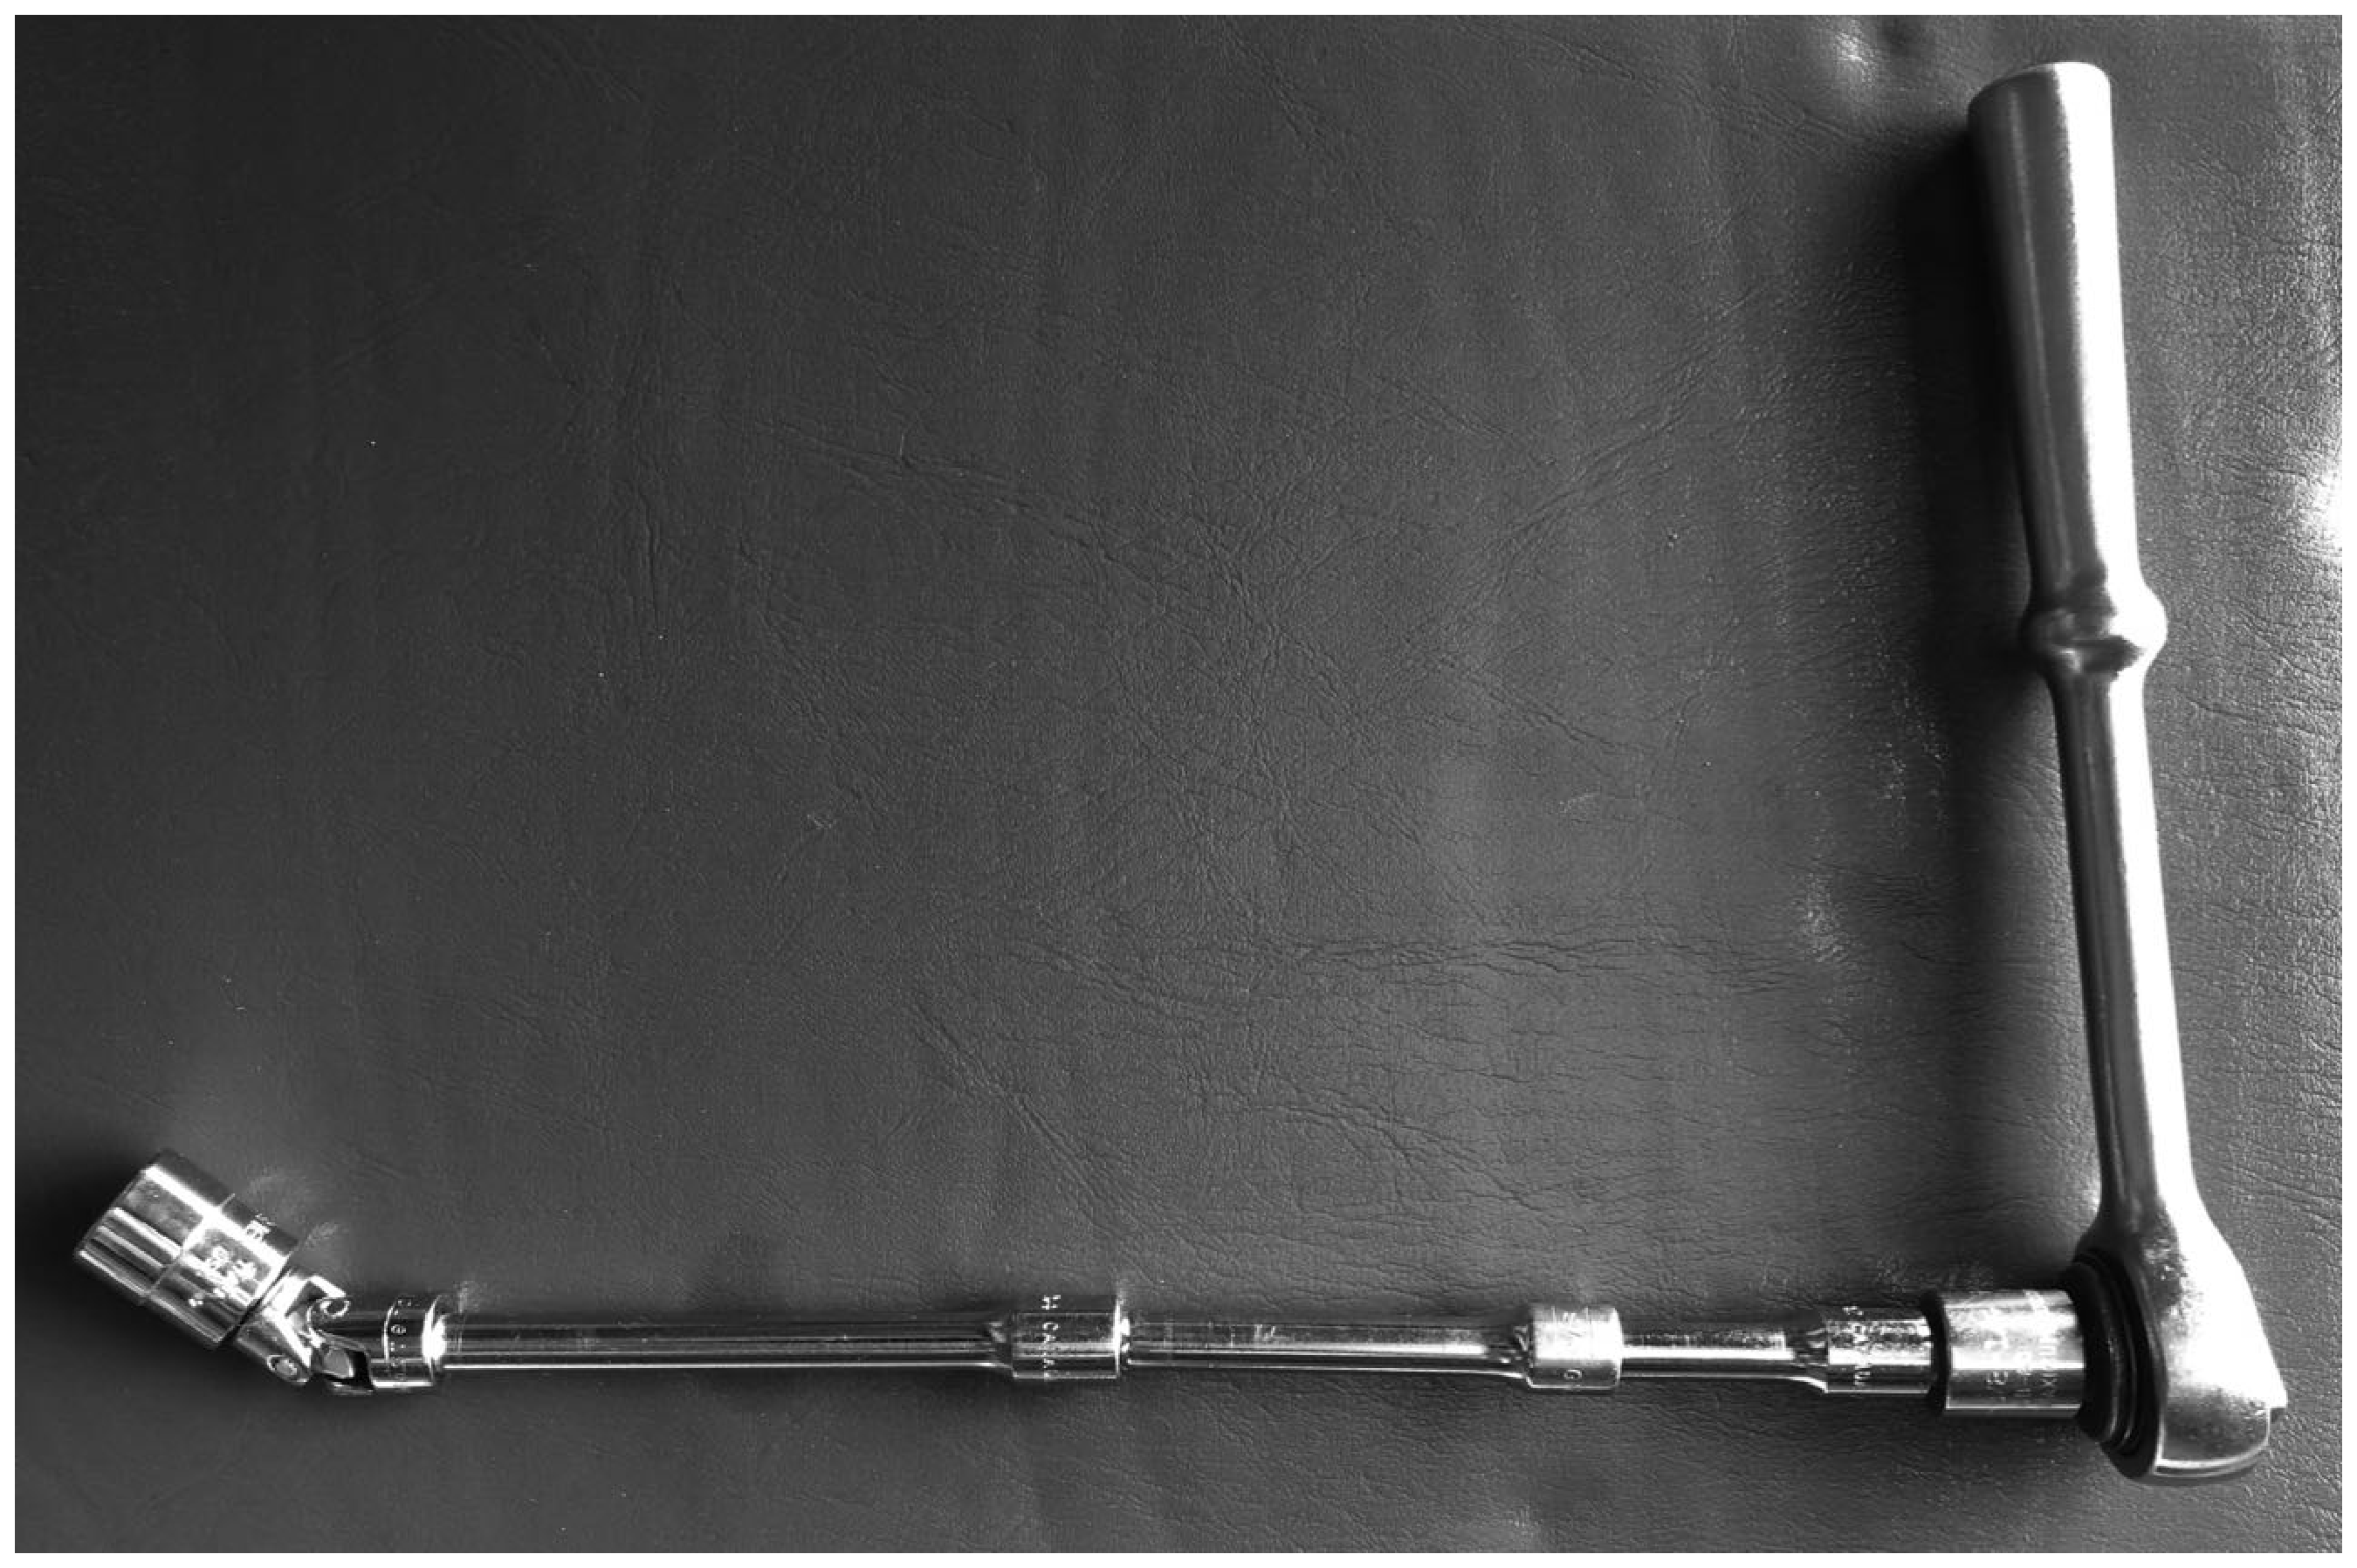
\includegraphics[scale=0.2]{../Diagrams/LG_Box_Fwd}
\end{center}
\caption{Tools for Forward Outboard LG Box Bolts (9/16" Socket)}
\end{figure}

\begin{figure}
[htb]
\begin{center}
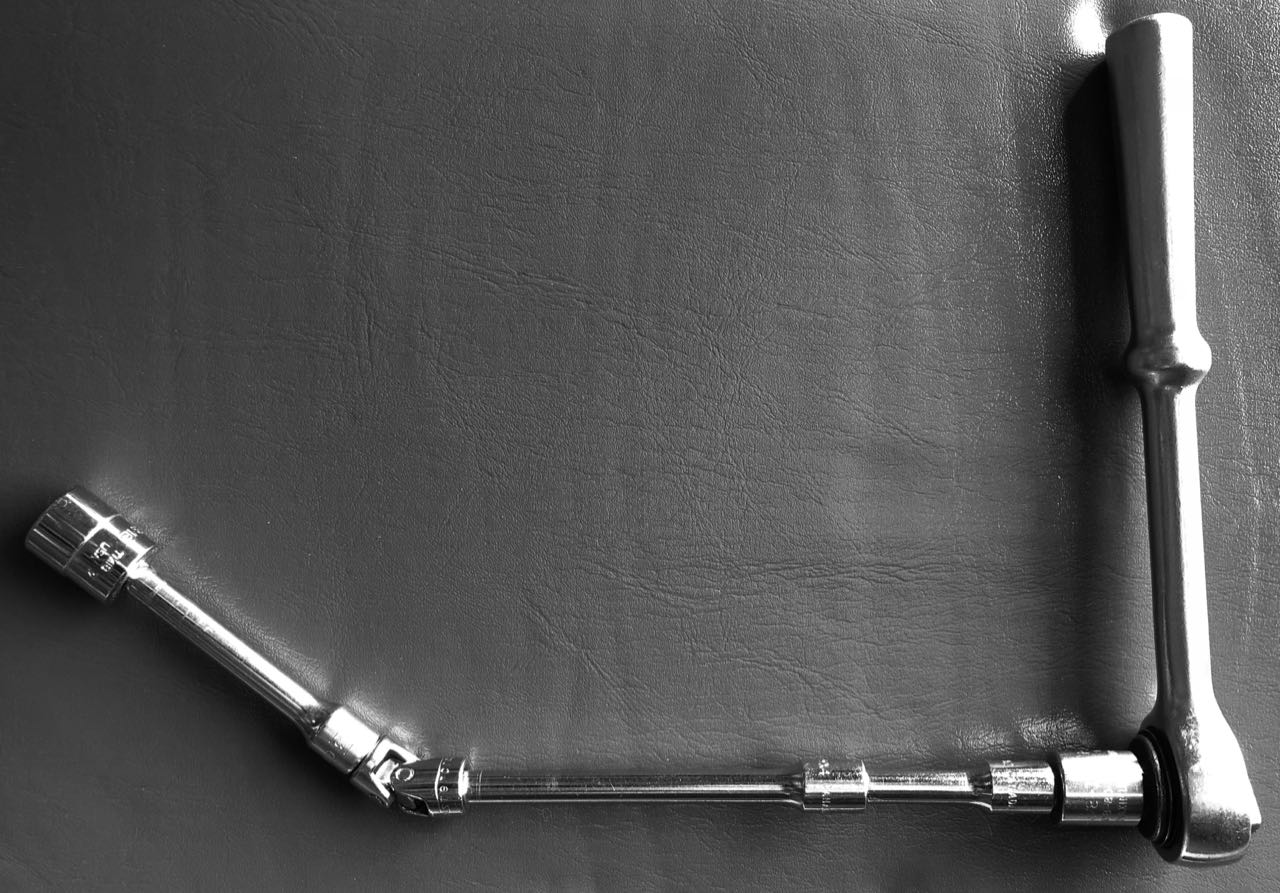
\includegraphics[scale=0.2]{../Diagrams/LG_Box_Aft}
\end{center}
\caption{Tools for Aft Outboard LG Box Bolts (9/16" Socket)}
\end{figure}

\section{JACK AIRCRAFT}
  \begin{enumerate*}
  	\item Remove wheel pants
    \item Insert jack post into socket on jack base
    \item Place lifting point on jack underneath the bottom of the landing gear leg, with the jack post on the inboard side of the landing gear leg
    \item Place securing arm between aft side of landing gear leg and brake caliper (move securing arm to other side of jack if needed)
    \item Tighten bolt that attaches securing arm to jack
    \item Use socket and ratchet to turn jack screw to raise jack
  \end{enumerate*}

\begin{figure}
[htb]
\begin{center}
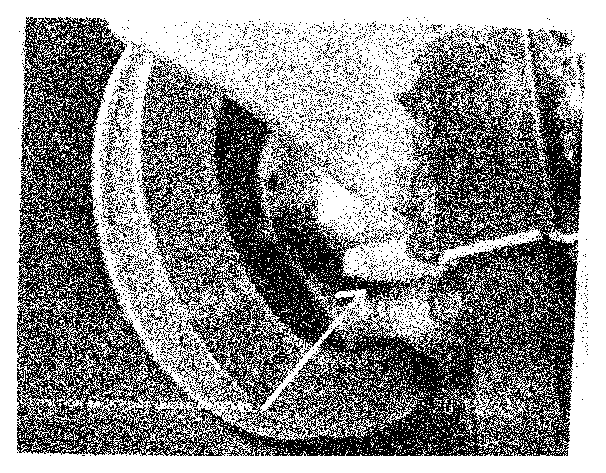
\includegraphics[scale=1]{../Diagrams/Jack_Instructions_1}
\end{center}
\caption{Jack lifting point under bottom of LG leg}
\end{figure}

\begin{figure}
[htb]
\begin{center}
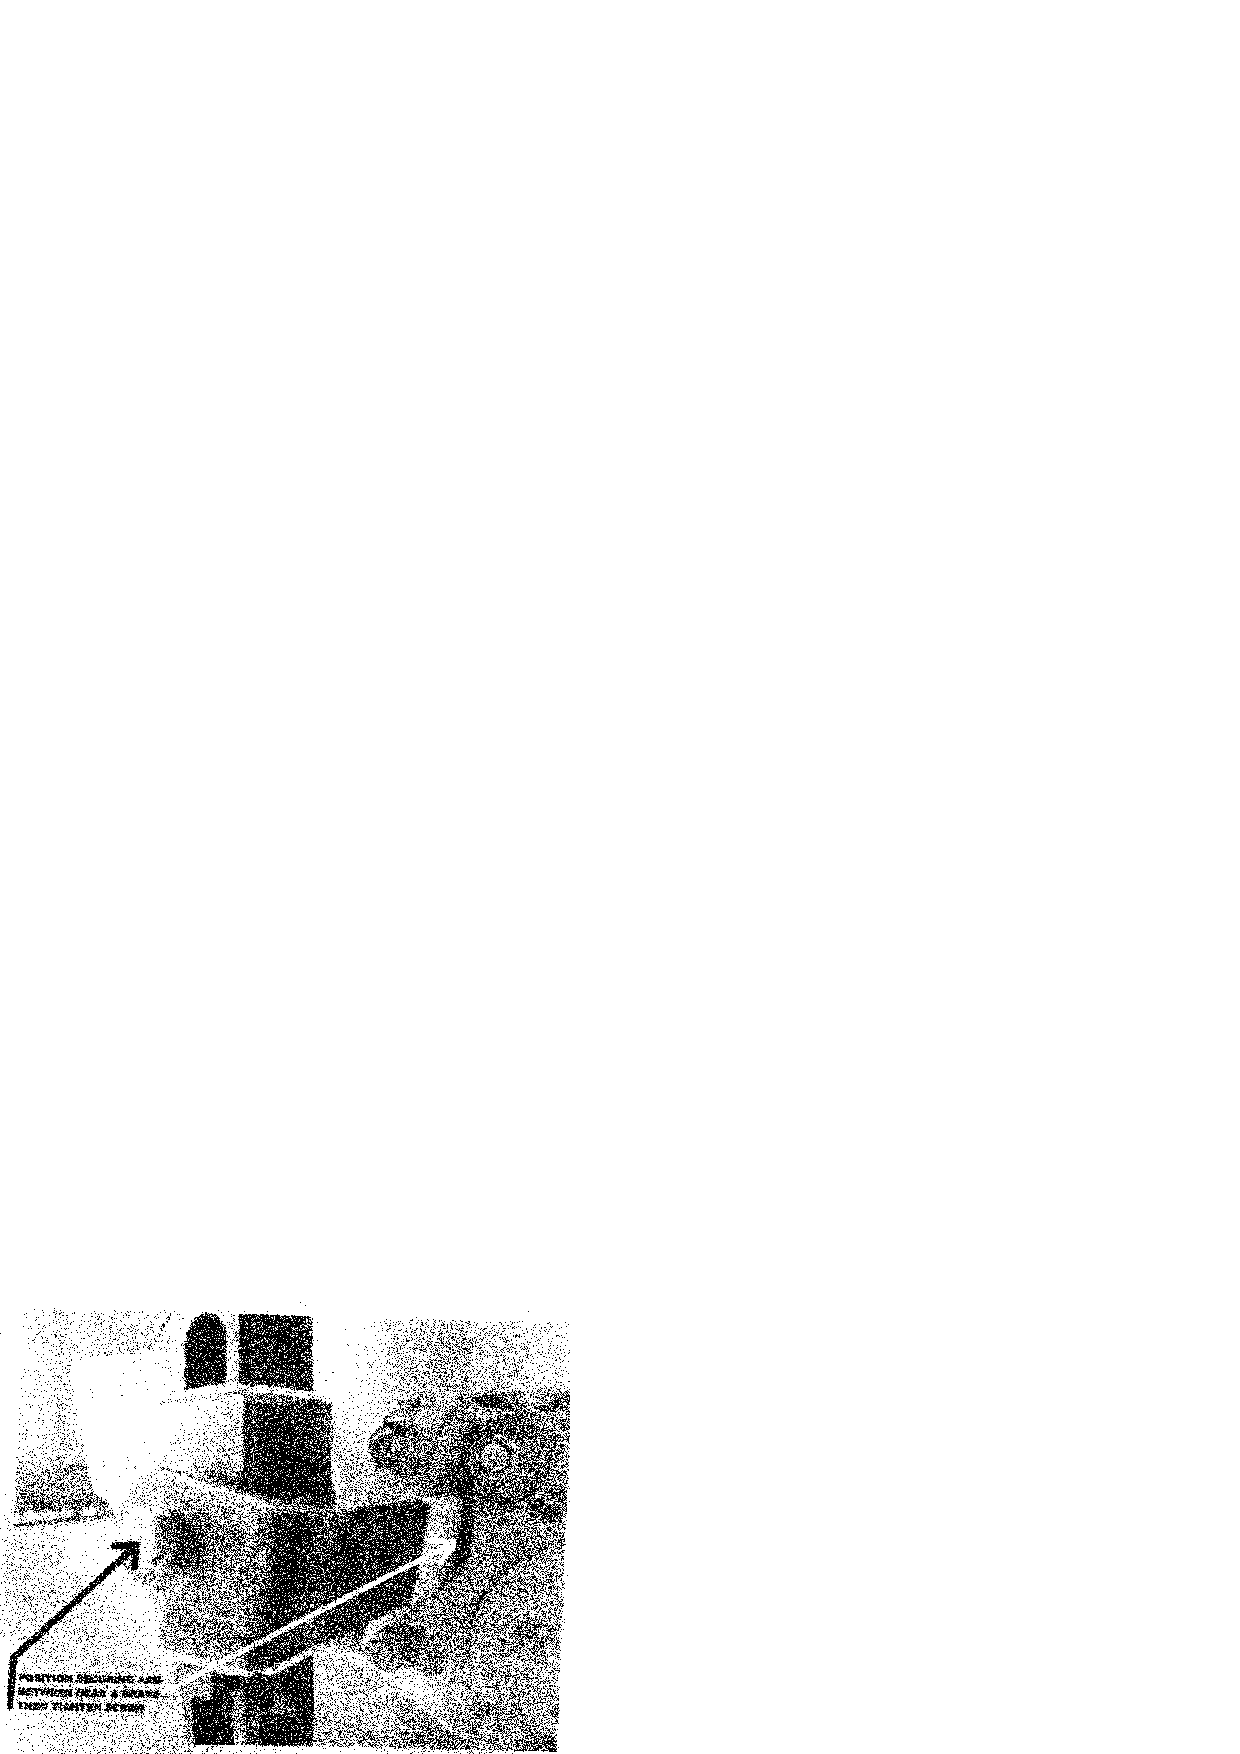
\includegraphics[scale=1]{../Diagrams/Jack_Instructions_2}
\end{center}
\caption{Securing arm between LG leg and brake caliper}
\end{figure}

\clearpage

\section{GNS 430W CONFIGURATION}
\begin{tabularx}{\textwidth} {| >{\setlength\hsize{1.4\hsize}}Y | >{\setlength\hsize{0.8\hsize}}Y | >{\setlength\hsize{0.8\hsize}}Y | c |} 
	\hline Section & Item & Value & Remarks\\
	\hline 
	\hline Main ARINC 429 Config        & IN 1                       & Speed: High         &\\
	                                    &                            & Data: OFF           &\\
	                                    & IN 2                       & Speed: High         &\\
	                                    &                            & Data: OFF           &\\
	                                    & OUT                        & Speed: High         &\\
	                                    &                            & Data: ARINC 429     &\\
	                                    & SDI                        & Common              &\\
	                                    & VNAV                       & Enable Labels       &\\
	\hline Main RSS Config              & Chnl 1                     & Input: Icarus Alt   &from GTX327\\
	                                    &                            & Output: OFF         &\\
	                                    & Chnl 2                     & Input: OFF          &\\
	                                    &                            & Output: ADS-B OUT + &to ADS-B\\
	                                    & Chnl 3                     & Input: OFF          &\\
	                                    &                            & Output: Aviation    &to AFCS and EFIS\\
	                                    & Chnl 4                     & Input: OFF          &\\
	                                    &                            & Output: OFF         &\\
	\hline Main System Config           & Configure                  & Fuel                &\\
	                                    & Fuel Type                  & Av Gas              &\\
	\hline Main System Config           & Configure                  & Discretes           &\\
	                                    & GPS Select                 & Auto                &\\
	                                    & COM Presets                & Enabled             &\\
	\hline COM Setup                    & Spacing                    & 25.0 kHz            &\\
	\hline Main Lighting                & Display Source             & 14V DC              &\\
	                                    & Key Source                 & Photo               &\\
	                                    & Display Resp Time/Min      & 4 / 080             &\\
	                                    & Key Resp Time/Min          & 4 / 40              &\\
	                                    & Display Slope/Offset       & 50 / 50             &\\
	                                    & Key Slope/Offset           & 50 / 50             &\\
	                                    & Key Slope/Offset           & 50 / 50             &\\
	                                    & Display Photo Trans \%     & 05                  &\\
	                                    & Display Photo Slope/Offset & 50 / 50             &\\
	\hline COM Setup                    & S250                       & 15                  &\\
	                                    & S833                       & 20                  &\\
	                                    & Side                       & 31                  &\\
	                                    & Mic                        & 44                  &\\
	\hline VOR/LOC/GS ARINC 429 Config  & Speed                      & RX: Low             &\\
	                                    &                            & TX: Low             &\\
	                                    & SDI                        & VOR/ILS 1           &\\
	                                    & DME Mode                   & Directed Freq 1     &\\
	\hline GPS Vertical Offset          & GPS Antenna Height         & 4 ft                &\\
	\hline 
\end{tabularx}
\clearpage


\section{uAVIONICS EchoUAT ADS-B CONFIGURATION}
\begin{tabularx}{\textwidth} {| >{\setlength\hsize{1.1\hsize}}Y | >{\setlength\hsize{1.1\hsize}}Y | >{\setlength\hsize{0.8\hsize}}Y | c |} 
	\hline Section & Item & Value & Remarks\\
	\hline 
	\hline Transceiver Config           & Control                                        & UAT TX Enabled       &\\
	                                    & ICAO Number                                    & C067BD               &\\
	                                    & Call Sign                                      & CGNHK                &\\
	                                    & Flight Plan ID                                 & left blank           &\\
	                                    & CSID Logic                                     & Enabled              &\\
	                                    & Anonymous Mode                                 & Disabled             &\\
	                                    & Emitter Category                               & Light Airplane       &\\
	                                    & VFR Code                                       & 1200                 &\\
	                                    & ADS-B IN Capability                            & Both 1090/978 MHz    &\\
	                                    & VSO                                            & 40                   &\\
	                                    & Aircraft Length (m)                            & L$\leq$15            &\\
	                                    & Aircraft Width (m)                             & W$\leq$23            &\\
	                                    & GPS Antenna Offset Lateral (m)                 & 0                    &\\
	                                    & GPS Ant Offset from nose (m)                   & 4                    &\\
	\hline Installation                 & Setup Source                                   & App (WiFi) Stored    &\\
	                                    & Control Source                                 & Transponder Monitor  &\\
	                                    & GPS Source                                     & External GPS (COM 2) &\\
	                                    & Traffic Uplink Output                          & MFD (COM 2)          &Not Connected\\
	                                    & COM 1 Rate                                     & 38400                &Not Connected\\
	                                    & COM 1 Data                                     & 810                  &Not Connected\\
	                                    & COM 1 Phy                                      & RS-485 Terminated    &Not Connected\\
	                                    & COM 1 Protocol                                 & TMAP                 &Not Connected\\
	                                    & COM 2 Rate                                     & 9600                 &\\
	                                    & COM 2 Input Protocol                           & ADS-B+               &\\
	\hline Advanced                     & Transponder Threshold                          & 1450                 &Reduced from default\\
	(Double Tap 'echo' at               &                                                &                      &value of 1550 to\\
	top of Echo iOS App                 &                                                &                      &improve Pressure\\
	to see Advanced options)            &                                                &                      &Altitude detection\\
	\hline 
\end{tabularx}
\clearpage

\section{GARMIN GTX-327 CONFIGURATION}
\begin{tabularx}{\textwidth} {| >{\setlength\hsize{1.1\hsize}}Y | >{\setlength\hsize{1.1\hsize}}Y | >{\setlength\hsize{0.8\hsize}}Y | c |} 
	\hline Section & Item & Value & Remarks\\
	\hline 
	\hline Display Mode                 & Display Mode                                   & AUTO                 &\\
	                                    & Level                                          & 85                   &\\
	\hline Backlight                    & BKLT                                           & MAN                  &\\
	                                    & LVL                                            & ----                 &Current Value\\
	                                    & RSP TIME                                       & 1                    &\\
	                                    & MIN                                            & 10                   &\\
	                                    & BKLT SRCE                                      & PHOTO                &\\
	                                    & SLOPE                                          & 50                   &\\
	                                    & OFFSET                                         & 50                   &\\
	\hline Key Lighting                 & KEY                                            & AUTO                 &\\
	                                    & LVL                                            & ----                 &Current Value\\
	                                    & RSP TIME                                       & 1                    &\\
	                                    & MIN                                            & 10                   &\\
	                                    & KEY SRCE                                       & PHOTO                &\\
	                                    & SLOPE                                          & 50                   &\\
	                                    & OFFSET                                         & 50                   &\\
	\hline 
\end{tabularx}

\section{TRIO PRO PILOT AUTOPILOT CONFIGURATION}
\begin{tabularx}{\textwidth} {| >{\setlength\hsize{1.1\hsize}}Y | >{\setlength\hsize{1.1\hsize}}Y | >{\setlength\hsize{0.8\hsize}}Y | c |} 
	\hline Section & Item & Value & Remarks\\
	\hline 
	\hline Config Settings              & HNAV Servo Position                            & 7916                 &\\
	                                    & HNAV Servo Direction                           & NM                   &\\
	                                    & VNAV Servo Direction                           & RV                   &\\
	                                    & AS/VS Select                                   & AS                   &\\
	                                    & Max Turn Rate                                  & Auto                 &\\
	                                    & Circle Last Waypoint                           & No                   &\\
	                                    & Default Vertical Rate                          & 500                  &\\
	                                    & AP Disconnect Mode                             & HNAV \& VNAV         &\\
	                                    & LED Flash Mode                                 & Fast Flash           &\\
	                                    & Zero Flight Data on Power Up                   & No                   &\\
	\hline Autopilot Preferences        & Backlight                                      & 9                    &\\
	                                    & Contrast                                       & (Blank)              &\\
	                                    & HNAV TRK Gain                                  & 3                    &\\
	                                    & HNAV CRS Gain                                  & 4                    &\\
	                                    & HNAV PI Gain                                   & 9                    &\\
	                                    & HNAV Servo Gain                                & 35                   &\\
	                                    & VNAV Servo Gain                                & 16                   &\\
	                                    & VNAV AH Gain                                   & 60                   &\\
	                                    & VNAV VS Gain                                   & 50                   &\\
	                                    & VNAV AS Gain                                   & 35                   &\\
	                                    & VNAV Servo Deadband                            & 4                    &\\
	\hline 
\end{tabularx}


\clearpage

\section{TORQUE TABLE} 
\begin{tabularx}
	{
	\textwidth}{|>{\setlength\hsize{.9\hsize}}Y|c|>{\setlength\hsize{1.1\hsize}}Y|} \hline Item&Torque Value&Remarks\\
	\hline \hline Main Alternator Mount&110 -- 150 in-lb&from Installation Instructions\\
	\hline Main Alternator Tension Arm&110 -- 150 in-lb&from Installation Instructions\\
	\hline Main Alternator Pivot Bolt&30 -- 40 ft-lb&from Installation Instructions\\
	\hline \ifthenelse{\thePMAG = 0}{Spark Plugs (Aviation)&35 ft-lb&from Lycoming Overhaul Manual\\
	\hline Spark Plugs (Automotive)&180 in-lb&from Electronic Ignition Installation Instructions\\}	
	{Spark Plugs&180 in-lb&from PMag and Electronic Ignition Installation Instructions\\}
	\hline \ifthenelse{\thePMAG = 1}{PMag Spark Plug Adapters&18 ft-lb&Screw adapters onto sparkplugs, and torque via the spark plug. Do no apply anti-seize. from PMag Installation Instructions\\
	\hline Light Speed Spark Plug Adapters&25 ft-lb&Do not apply anti-seize. from Electronic Ignition Installation Instructions\\}
	{\hline Light Speed Spark Plug Adapters&25 ft-lb&Do not apply anti-seize. from Electronic Ignition Installation Instructions\\}
	\hline Rocker Box Screws&50 in-lb&from Lycoming Overhaul Manual\\
	\hline Intake pipe bolts with silicone gaskets&15 in-lb&from Steve Mahoney\\
	\hline Exhaust Pipe Nuts&180 -- 200 in-lb&Apply anti-seize. from Vetterman Exhaust Installation Instructions\\
	\hline \ifthenelse{\thePMAG = 0}{Magneto}{PMag} and EI Hall Effect Unit Base Clamps&204 in-lb&from ECI Service Info\\
	\hline Propeller Governor Mounting Nuts&110 -- 150 in-lb&from PCU-5000 Installation and Adjustment document\\
	\hline Propeller Governor High RPM Stop Jam Nut&24.8 -- 28.3 in-lb&from PCU-5000 Installation and Adjustment document\\
	\hline Oil Screen&135\textdegree \ rotation after contact&from Lycoming SSP-1776-B\\
	\hline Propeller Hub&63 -- 66 ft-lb&from MT Operation and Installation manual\\
	\hline Spinner Screws&35 -- 44 in-lb&from MT Operation and Installation manual\\
	\hline Brake caliper bolts&75 -- 80 in-lb&from Cleveland service info\\
	\hline Wheel half bolts&90 in-lb&Bolts that join the two halves of each wheel. Value from Cleveland service info\\
	\hline Landing gear outboard 7/16" bolts&240 in-lb&from RV-8 Builder's Manual\\
	\hline Landing gear inboard 7/16" bolts&450 -- 500 in-lb&from AC43.13-1B\\
	\hline Landing gear inboard 5/16" bolts&100 -- 140 in-lb&from AC43.13-1B\\
	\hline 
\end{tabularx}

\clearpage
\section{FUSE BLOCKS}
\begin{figure}
  \centering
  % 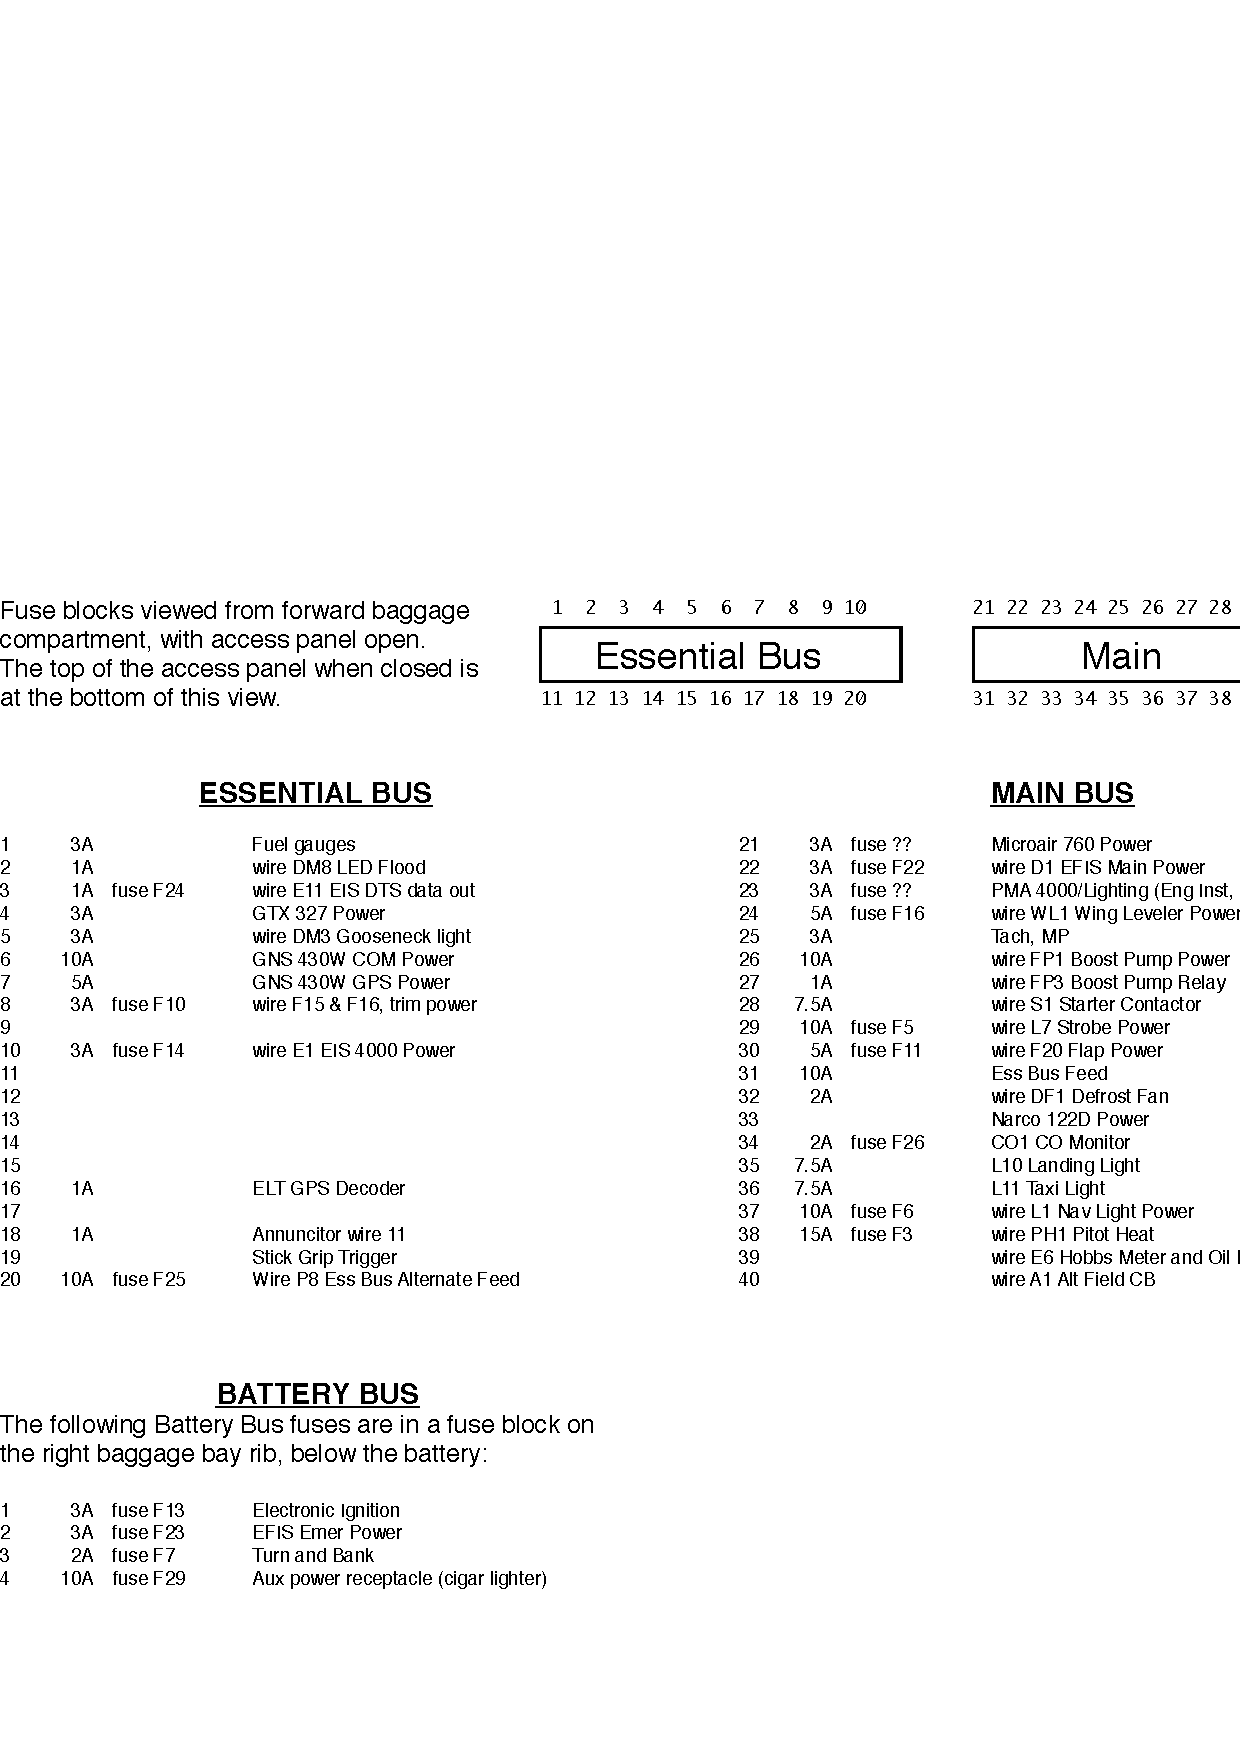
\includegraphics[width=1.1\textwidth, angle=90]{../Diagrams/Fuse_Blocks_POH}
  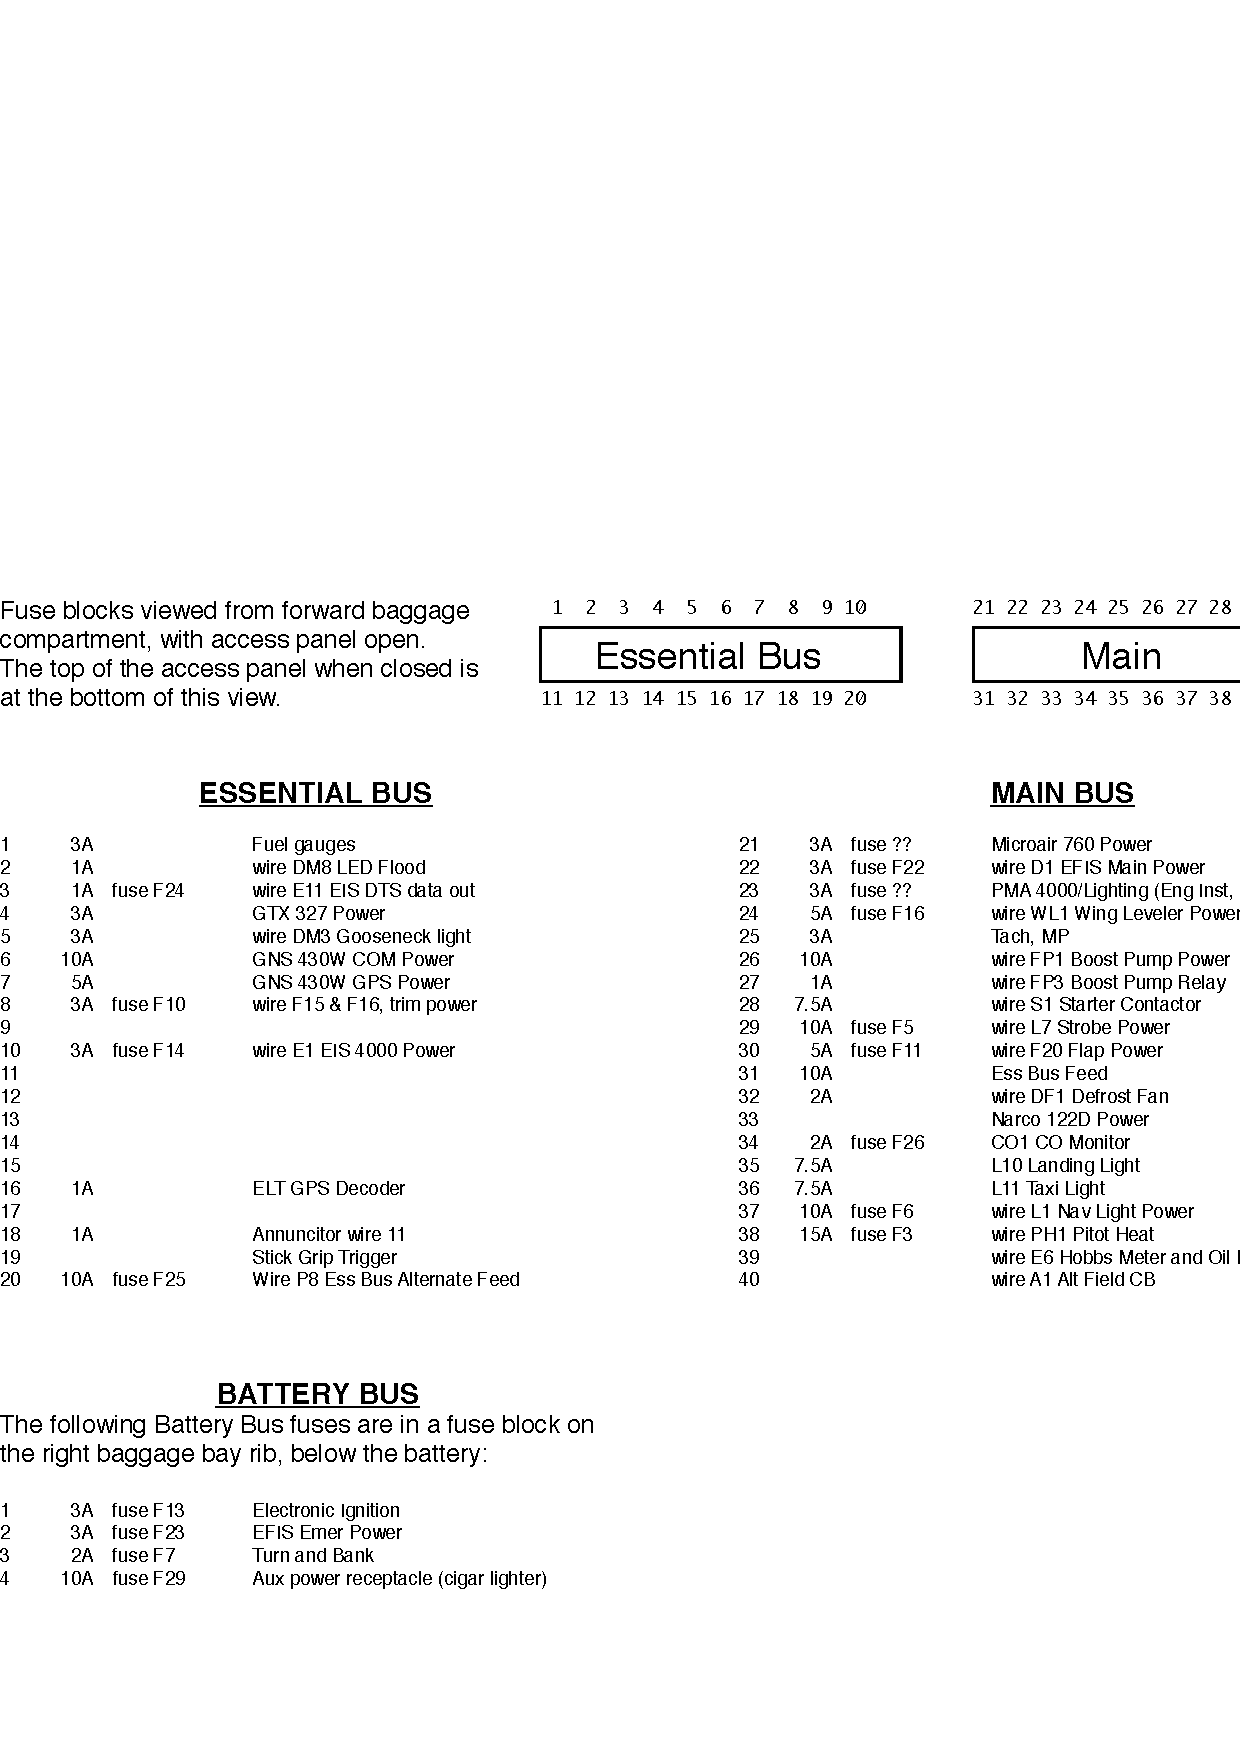
\includegraphics[width=1.2\textwidth, angle=90]{../Diagrams/Fuse_Blocks_POH}
  \label{fig:FuseBlocks}
  \caption{Fuse Blocks}
\end{figure}
\cleardoublepage 
